\documentclass{report}
\usepackage[utf8]{inputenc}     % for éô
\usepackage[english]{babel}     % for proper word breaking at line ends
\usepackage[a4paper, left=1.5in, right=1.5in, top=1.5in, bottom=1.5in]{geometry}
                                % for page size and margin settings
\usepackage{graphicx}           % for ?
\usepackage{amsmath,amssymb}    % for better equations
\usepackage{amsthm}             % for better theorem styles
\usepackage{mathtools}          % for greek math symbol formatting
\usepackage{varwidth}
\usepackage{enumitem}           % for control of 'enumerate' numbering
\usepackage{listings}           % for control of 'itemize' spacing
\usepackage{todonotes}          % for clear TODO notes
\usepackage[hidelinks]{hyperref}           % page numbers and '\ref's become clickable
\usepackage{pgfplots}
\usepackage{caption}
\usepackage{parskip}
\usepackage{makecell}
\usepackage{tabularx} 

% \pgfplotsset{width=10cm,compat=1.9}


% Listing style

%% Package for colors.
\usepackage{xcolor}
%% Useful colors
\definecolor{blue}{RGB}{0,0,255}
\definecolor{codegreen}{rgb}{0,0.6,0}
\definecolor{codegray}{rgb}{0.5,0.5,0.5}
\definecolor{codepurple}{rgb}{0.58,0,0.82}
\definecolor{backcolour}{rgb}{1,0.973,0.906}
\definecolor{mygray}{gray}{0.96}

%% Code listing style named "mystyle"
\lstdefinestyle{mystyle}{
  backgroundcolor=\color{mygray},
  %commentstyle=\color{codegreen},
  %keywordstyle=\color{magenta},
  %numberstyle=\tiny\color{codegray},
  stringstyle=\color{codepurple},
  basicstyle=\footnotesize,
  breakatwhitespace=false,         
  breaklines=true,                 
  captionpos=b,                    
  keepspaces=true,                 
%   numbers=left,                    
  numbersep=5pt,                  
  showspaces=false,                
  showstringspaces=false,
  showtabs=false,                  
  tabsize=2
}
% "mystyle" code listing set
\lstset{style=mystyle}


%%%%%%%%%%%%%%%%%%%%%%%%%%%%%%%%
%% SET TITLE PAGE VALUES HERE %%
%%%%%%%%%%%%%%%%%%%%%%%%%%%%%%%%
%             ||               %
%             ||               %
%             \/               %

\def\thesistitle{WIP Authenticated video calling}
\def\thesissubtitle{The need for authenticated video calling}
\def\thesisauthorfirst{Julian van der Horst \\ s1015357}
\def\thesisauthorsecond{}
\def\thesissupervisorfirst{Bart Jacobs}
\def\thesissupervisorsecond{Omar Javed}
\def\thesissecondreaderfirst{TBA}
\def\thesissecondreadersecond{}
\def\thesisdate{May 2023}


%% FOR PDF METADATA
\title{\thesistitle}
\author{\thesisauthorfirst\space\thesisauthorsecond}
\date{\thesisdate}

%%%%%%%%%%%%%%%%%%%%%%%

\begin{document}
\begin{titlepage}
	\thispagestyle{empty}
	\newcommand{\HRule}{\rule{\linewidth}{0.5mm}}
	\center
	\textsc{\Large Radboud University Nijmegen}\\[.7cm]
	
\includegraphics[width=25mm]{img/in_dei_nomine_feliciter.eps}\\[.5cm]
	\textsc{Faculty of Science}\\[0.5cm]
	
	\HRule \\[0.4cm]
	{ \huge \bfseries \thesistitle}\\[0.1cm]
	\textsc{\thesissubtitle}\\
	\HRule \\[.5cm]
	\textsc{\large Thesis MSc Computing Science}\\[.5cm]
	
	\begin{minipage}{0.4\textwidth}
	\begin{flushleft} \large
	\emph{Author:}\\
	\thesisauthorfirst\space \textsc{\thesisauthorsecond}
	\end{flushleft}
	\end{minipage}
	~
	\begin{minipage}{0.4\textwidth}
	\begin{flushright} \large
	\emph{Supervisor:} \\
	\thesissupervisorfirst  \\[1em]
    \emph{Daily supervisor:} \\
    \thesissupervisorsecond \\[1em]
	\emph{Second reader:} \\
	\thesissecondreaderfirst\\ 
    % \thesissecondreadersecond
	\end{flushright}
	\end{minipage}\\[4cm]
	\vfill
	%{\large \thesisdate}\\
	{\large \today}\\
	\clearpage
\end{titlepage}

\tableofcontents

\newpage
\section*{Abstract}

\chapter{Introduction}


\chapter{Background}
We will make use of existing tools to build functionality in to pubhubs. We will need to introduce some background information first. 

\section{PubHubs}
PubHubs, short for Public Hubs, is an alternative community platform that puts public values first \cite{jacobs_pubhubs_2023}. Unlike mainstream social media platforms like Instagram or Twitter that focus on individual broadcasting, PubHubs emulates real-world social dynamics by centering interactions within smaller, community-based hubs. The reasoning behind that is that this behavior closely resembles normal human interaction, where humans have small groups of friends and collaborators with whom they interact. The way people experience social media now is very unnatural, where if they engage with a platform, their posts are shouted into the whole world and are for everyone to see.

“PubHubs is organized as a network of independent hubs, with a shared single-sign-on. Conversations take place in local hubs (and not globally) and the associated (conversation) data is managed decentrally, within each hub” \cite{jacobs_pubhubs_2023}. Privacy is one of the core values of PubHubs, which can be seen in how it handles identity management. The main idea of Pubhubs is to allow pseudonymity while maintaining both accountability and the ability to verify certain attributes of the user. The authentication of users is done using Yivi (formerly IRMA)\cite{alpar_irma_nodate} and the identity (the pseudonym) is generated using PEP \cite{verheul_polymorphic_2016}. In PubHubs all communication is done via Matrix. “Matrix is an open-source network for secure, decentralized communication” \cite{noauthor_matrixorg_nodate}.

Pubhubs uses a prvacy first design where attributes can be disclosed if the user so chooses. This approach we will use in our design of the video conferencing feature.

\section{Video conferencing}
During the COVID-19 pandemic, there was a big need for remote work. Immediately, services like Zoom \cite{Zoom}  and Microsoft Teams  \cite{MSTeams} gained widespread adoption. These tools allowed video conferencing between different remote locations in real-time. These video call services might include end-to-end encryption but often lack authenticated video conferencing. Perhaps the need for authenticated video conferencing is not very apparent, and when calling friends it might not be needed. In contrast, when having an online consultation with your doctor, you want to be sure that you are actually calling a doctor.

% Misschien een sectie waar we vertellen dat je nu met AI heel veel dingen kan faken?

If we look at video conferencing from a conceptual perspective, we see that there are multiple conferencing setups. For this research, we will distinguish three types. Person-to-person (one-on-one), Person-to-person (multiple people), and speaker-to-audience. We distinguish these types because they all have certain properties that best match with different technologies. Where in one-on-one we only need to send and receive to one other person, when we are in a group we need to send and receive data to each member in a call. On the contrary, with speaker-to-audience, we do not have connections between the individual audience members. The first and second setup are more in line with what we expect the users of Pubhubs to use video conferencing for, so we will focus on them in this research. 

\begin{figure}[!hbt]
    \centering
    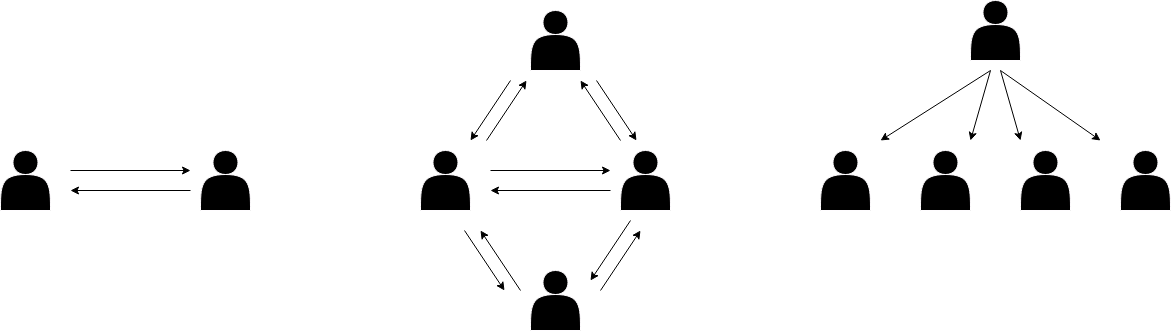
\includegraphics[width=0.7\textwidth]{Research proposal/img/three types.drawio.png}
    \caption{The three types of video conferencing}
    \label{fig:enter-label}
\end{figure}

With video conferencing, people need to send and receive video streams, and we want to do this ideally in real time. A standard for that is WebRTC, and it is now widely supported in browsers (97.77\%) \cite{CIUIWEBRTC}. WebRTC is both a protocol and an API that can be used for many things, including video and audio communication. Matrix even has support for WebRTC and uses it in their main testing application Element \cite{ELEMENT}. In our implementation, we will use WebRTC to send video and audio streams. However, to which endpoints do we need to send these WebRTC streams?

The first option is to send the data in a Peer-to-peer (P2P) network. This means that the people in the call send their stream to every other person in the call. This ensures that the server has no extra load since it does not handle any video streams, it simply facilitates the call setup. However, with every extra participant, every user needs to send/receive more and more data. At some point, a bottleneck is reached, and no extra participant can be added or a loss in data will occur. This is a very privacy-friendly method since the server has no access to the video conferencing data being sent and the users have full autonomy to choose who can receive their video data. However, due to the limited number of participants, this solution is not feasible.

Another option would be to have a Multipoint Control Unit (MCU). An MCU takes in many media streams and combines them into one media stream. This makes it so that it can work very well with legacy systems, since an MCU can receive various types of media and then output a standardized output. For example, this would allow a participant to call in from a phone connection while the other participant have a video call. The MCU has to decode all the incoming media signals, which makes it costly at large scale, since the CPU usage would be very high. From a security and privacy perspective, this solution is not ideal, since the server has access to all the unencrypted video and audio data. 

Lastly, we have the Selective Forwarding Unit (SFU). An SFU behaves in a way like a switch where it would selectively forward streams between clients, it does not interact with the video streams so it would work similarly with encrypted and unencrypted data. From a user perspective, we only need to talk to one server, and we send and receive all our data through that server. An SFU provides a compelling balance of scalability and privacy. it needs lower resources since it only needs to forward the signals to the users and does not decrypt the data. 

\section{Matrix and Element call}
As mentioned previously, Pubhubs uses Matrix when sending messages. Matrix not only used in sending messages and multimedia between users, but it is fundamentally used to create and manage the rooms in Pubhubs. Thus, when creating the architecture and prototype, the matrix protocol should be considered as to not make choices which directly oppose the matrix standard. The community can suggest changes to the Matrix protocol by submitting proposals, and over the years this has added a lot of functionality to Matrix. In proposal 3401 \cite{MATRIX_VIDEO_CALL_PROP}, functionality for video conferencing was proposed. This proposal can be applied to all the above-mentioned server setups and describes a protocol for video conferencing. 

The same team that built matrix is also building Element \cite{ELEMENT}, which is an open-source implementation of a messaging app that uses matrix. A new feature was added to Element called Element call, which serves as an example implementation of the proposal mentioned above. They started by using peer-to-peer video conferencing, since this more closely resembled the decentralized infrastructure of Matrix. However, this turned out to not be the best solution since it allowed for a maximum of 7 participants and video conferencing required numerous computer resources from participants. Recently, they have released a new version that makes use of an open-source SFU called Livekit \cite{LIVEKIT}.

We will use this implementation as a guide during our research; however, we will evaluate all the different choices made for Element call and deviate from them based on the requirements of PubHubs. When using Livekit we can easily implement features like noise suppression or video simulcast (Sending multiple video streams with different qualities, to dynamically choose the quality according to a user's internet connection).

\chapter{Current privacy considerations}
\section{Separation of the client}
Pubhubs currently has  a strong divide between Pubhubs central and different hubs. Pubhubs central knows your identity, whereas the hubs know your local identity and the messages you send there. This division is even made in the client, where there is a distinction of the global and the hub client. 

The global client, enables a user to go from hub to hub and log in. This is the area that Pubhubs has full control over, so ideally this client should not infer any information about your behavior in hubs. The global client enables Pubhubs to have a global login and enables the user to quickly switch between hubs, without reloading or logging in again. The hub client is what the hub itself actually deploys. Here, hubs can create rooms or add plugins. This hub only knows your local identity, but it should not be able to read your data or identity from other hubs. When you load Pubhubs from your browser, you visit the global client, where you log in. To interact with a hub, the global client loads the hub client in an Iframe, creating a barrier between the global and hub client. 

The Iframe has the sandbox attribute set, meaning that some browser features cannot be accessed from within the iframe. This turned out to be a problem, when requesting Camera and Microphone access, since these are considered secure attributes. We can request these permissions in the global client; however, this does in essence allow the hub client to identify the users across hubs. The hub can create a profile of users by saving which video conferencing devices are connected. We could perhaps work out a way to spoof the names of the devices, but this would impact the user experience by making it difficult to see which device is your preferred one.

\todo{Andere manieren van user profile building}
\todo{Device spoofing maybe}


\chapter{Proposed solution}

\begin{figure}
    \centering
    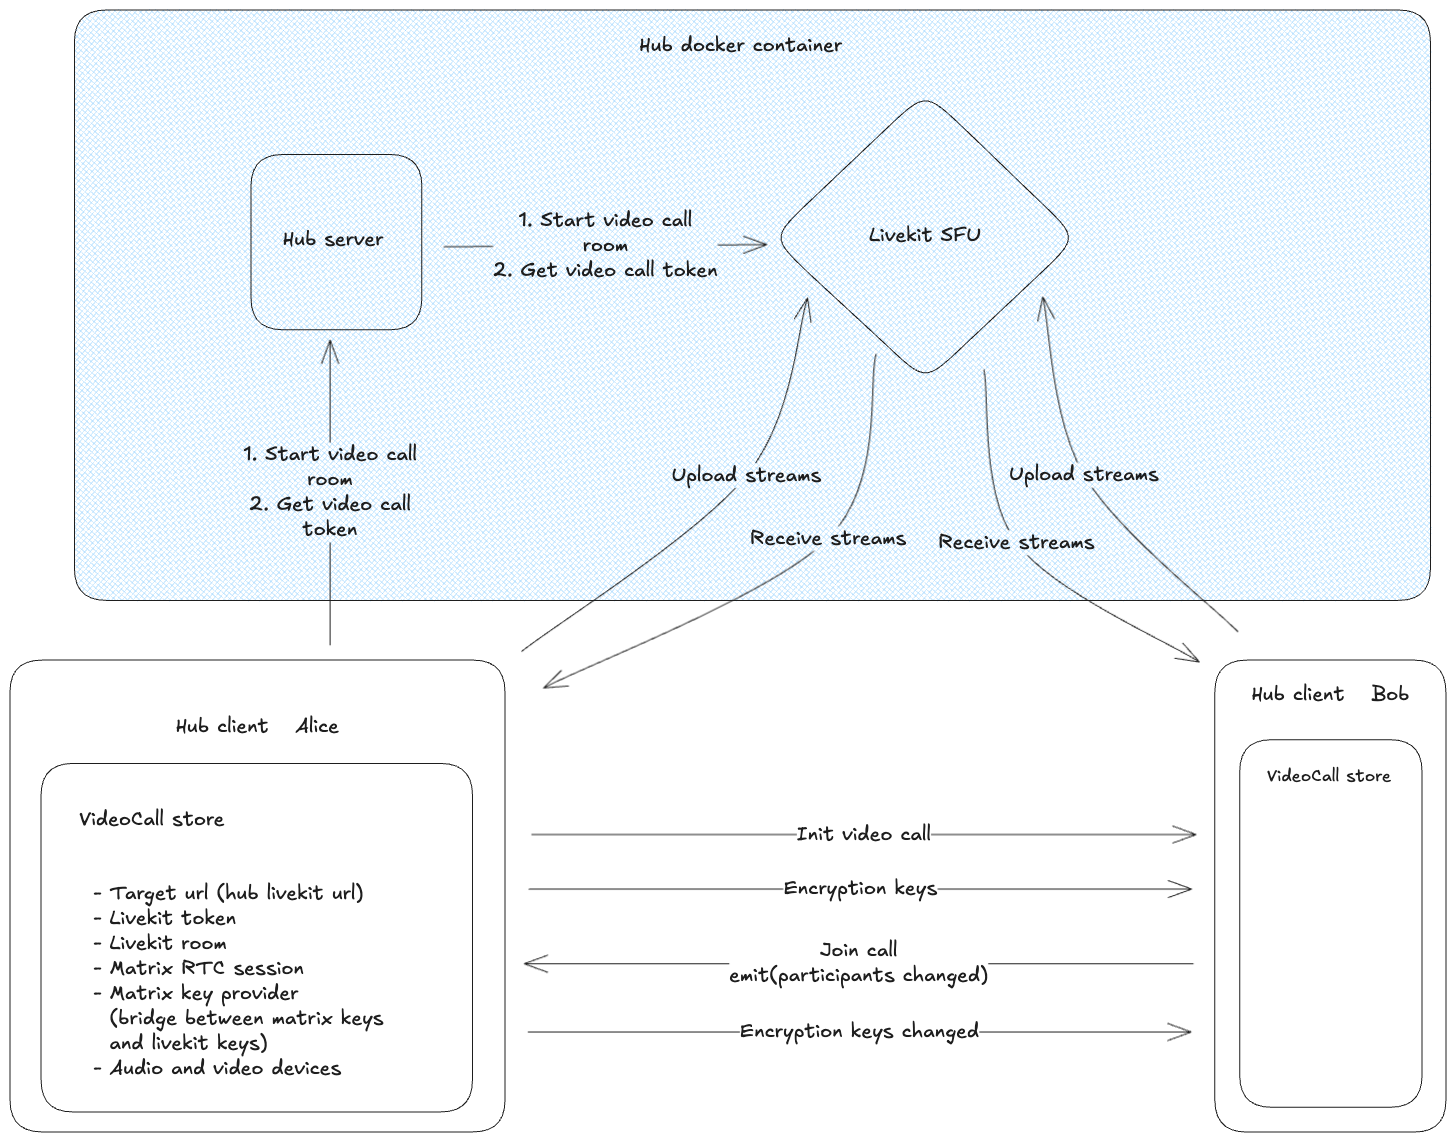
\includegraphics[width=\textwidth]{Master thesis/img/PH_videocall.excalidraw.png}
    \caption{Caption}
    \label{fig:enter-label}
\end{figure}
We first consider the Hub server, which will now also need to deploy a Livekit server instance. This livekit server functions as an SFU and will forward all the video and audio traffic between the different clients. This server will not see the video data which is sent since they are encrypted and the server does not have access to the keys. The only thing that the livekit server sees it the local pseudonym of the user, which the hub server already knows and thus does not leak additional data. The hub server authenticates the user by checking the authentication token on the request. These tokens are again the same as when 




. The response of this call will be the video call token from livekit for this pseudonym and for this room. 

The user then has the livekit token, which it will provide when uploading data to the SFU. Non authenticated media will be rejected \todo{Test this}. This flow is separated from the video conferencing room infrastructure. This is according to the new matrix spec done on Matrix itself. Recently, Matrix has changed its spec to let all the media handling be done outside of matrix and only concern matrix with setting up a room and sending invitations to the participants. So the only messages that are being sent over matrix are:

\begin{itemize}
    \item Init video call
    \item My encryption keys
    \item Join video call messages
    \item New encryption keys
\end{itemize}

This setup can be fully removed from a hub, should a hub not want video conferencing. It is standing on its own and can be toggled on or off using a flag. Everything is programmed in such a way that it is completely isolated from the rest of Pubhubs. 

\section{Encryption}

For video calling, we want to have end-to-end encryption. This encryption should ideally also have forward secrecy. Meaning that new participants cannot decrypt previous messages. Livekit provided an e2ee worker, which locally encrypts and decrypts incoming messages. For that, we do need the keys from all participants. Matrix is now in the middle of transitioning to a new spec where the client can more directly request, revoke and rotate keys of the participants.

We subscribe to a Matrix\_RTC\_Session. This will give us messages when a new user is added or when the keys are updated. Whenever we get an updated key message from the rtc\_session, we pass it through livekit, which in turn updates the keys and derives new keys from that key. It simply takes the key from matrix\_rtc and uses that as a seed.

Livekit uses AES-GCM, to encrypt the frames. This is a widely used and researched block cipher, meaning that once we have provided it with a key, we can have freshly encrypted video conferencing data. We chose to use the built-in encryption tools from matrix, this way we don't need to reinvent the wheel and add extra strain on the developers by developing a full-blown crypto system on top of the Pubhubs application.

Currently, the matrix team has enabled e2ee, but they used a now old C++ implementation of Olm. They are now moving toward their new Rust implementation of it. It is not completely up to par, but the features we need are here. We don't need much for the encryption of video calls, however, when we use the crypto library to create random keys which we will send and use to encrypt our sources.

% \newpage
% \section{Research question}
% The main research question will be \textbf{“How can we design and implement an authenticated video conferencing solution within PubHubs that balances privacy, security, and usability?”}. This main question creates several sub-questions. We will divide these up into three different categories.

% \textbf{Privacy}
% For Pubhubs privacy is one of their core values and during the creation and development of Pubhubs certain decisions have been made regarding privacy. These decision should be considered and can be formulated into these sub-questions:

% — What information or metadata should we allow leaking to achieve authenticated video conferencing, regarding the current Pubhubs privacy principles?

% — How can we balance essential call features, like visible call status, with a commitment to user privacy?

% \textbf{Encryption}
% One of the foremost considerations in GDPR compliance for video conferencing is the implementation of end-to-end data encryption. This requires an encryption scheme which is user-friendly, has low computational overhead, and still has appropriate security.

% — What encryption scheme is best suited for authenticated video conferencing in Pubhubs, weighing user experience and computational overhead while ensuring optimal security? 

% \textbf{Development}
% While doing the research and writing the code for it, we should also keep in mind the current development setup for PubHubs. This means that we should keep in mind which technologies they are using now and remain in those ecosystems. This makes it so that the code can be more easily maintained in the future. Pubhubs allows hubs to create their own version of the hub client, which should be considered when creating the video conferencing client.

% — How can we develop a video conferencing prototype within the existing Pubhubs ecosystem, while simultaneously considering different hub client implementations?

\bibliographystyle{plain}
\bibliography{references.bib}

\end{document}